\documentclass[tikz]{standalone}

\usepackage{xparse}
\usepackage{amsmath,amssymb}
\usepackage{tabularray}
\usepackage{enumitem}
\usepackage{unicode-math,float}
\usepackage{tikz}
\usepackage{varwidth}
\usepackage{fontspec}       

\UseTblrLibrary{varwidth}
\UseTblrLibrary{functional}

\usetikzlibrary{calc,shapes,arrows,positioning,patterns,fit,shapes.arrows, fadings,arrows.meta,automata}
    \usetikzlibrary{decorations.text,patterns.meta}
		\usetikzlibrary{decorations.pathmorphing,calc,shadows.blur,shadings,decorations, backgrounds,trees}
		\usetikzlibrary{matrix}
		\usetikzlibrary{intersections}
		\usetikzlibrary{animations} % LATEX and plain TEX
		\usetikzlibrary{mindmap}
		\pgfdeclarelayer{background}
		\pgfdeclarelayer{foreground}
		\pgfsetlayers{background,main,foreground}   %% some additional layers for demo

\usepackage{circuitikz}
\usepackage{polyglossia}
\usepackage{xfrac,unicode-math}
\newfontfamily\arabicfont[Script=Arabic,Scale=1]{Tahoma}
%RawFeature={-dlig,-ss02},
%\newfontfamily\englishfont[]{Naughty}
\newfontfamily\Trad[Script=Arabic]{Traditional Arabic}
\newfontfamily\Hfs[Script=Arabic]{Traditional Arabic}



%\newfontfamily\sevensegments[Scale=0.7]{DSEG7 Modern}
\newfontfamily\TahomaFont{Tahoma}

\newfontfamily\englishfont[Scale=1]{Tahoma}
%FF Yaseer
%\setmathfont[RawFeature={+ss01,-ssty}]{Naughty}

\setotherlanguage[numerals=maghrib]{arabic} %My main & native language
\setmainlanguage{english}


\newcommand{\rightbra}{{\Trad ﴿}}
\newcommand{\leftbra}{{\Trad ﴾}}

\newcommand{\addlab}[3]{%
	\\  #1 & #3 & #2
}

\makeatletter
\pgfset{
  /pgf/decoration/randomness/.initial=2,
  /pgf/decoration/wavelength/.initial=100
}
\pgfdeclaredecoration{sketch}{init}{
  \state{init}[width=0pt,next state=draw,persistent precomputation={
    \pgfmathsetmacro\pgf@lib@dec@sketch@t0
  }]{}
  \state{draw}[width=\pgfdecorationsegmentlength,
  auto corner on length=\pgfdecorationsegmentlength,
  persistent precomputation={
    \pgfmathsetmacro\pgf@lib@dec@sketch@t{mod(\pgf@lib@dec@sketch@t+pow(\pgfkeysvalueof{/pgf/decoration/randomness},rand),\pgfkeysvalueof{/pgf/decoration/wavelength})}
  }]{
    \pgfmathparse{sin(2*\pgf@lib@dec@sketch@t*pi/\pgfkeysvalueof{/pgf/decoration/wavelength} r)}
    \pgfpathlineto{\pgfqpoint{\pgfdecorationsegmentlength}{\pgfmathresult\pgfdecorationsegmentamplitude}}
  }
  \state{final}{}
}
\tikzset{xkcd/.style={decorate,decoration={sketch,segment length=0.5pt,amplitude=0.8pt}}}
\makeatother

\newcommand\rateme[1]{%
	\begin{tikzpicture}
		\fill (0,0) rectangle (#1*2.5/5,0.3);
		\draw (0,0) rectangle (2.5,0.3);
		\begin{scope}
			\clip (#1*2.5/5,0) rectangle (2.5,0.3);
			\node [inner sep = 0pt,scale=0.7] at (1.25,0.15) {$#1$};
		\end{scope}
		\begin{scope}
			\clip (#1*2.5/5,0) rectangle (0,.3);
			\node [inner sep = 0pt,scale=0.7,text=white] at (1.25,0.15) {$#1$};
		\end{scope}
		
	\end{tikzpicture}
}

%\newcommand{\SevenSeg}[1]{\textenglish{\sevensegments #1}}

\newcommand{\SevenSeg}[1]{\tikz[baseline=(A.base)]{
	\node [fill=red!25,text=red] (A) {\textenglish{\sevensegments #1}};
	%\node [text=red] (B) {\textenglish{\sevensegments #1}};
}}
\newcommand\MATHSPACE{%
\setlength{\belowdisplayskip}{0.0ex}%
\setlength{\belowdisplayshortskip}{0.5ex}%
\setlength{\abovedisplayskip}{0.5ex}%
\setlength{\abovedisplayshortskip}{0.5ex}%
}
\IfFileExists{\jobname.tempfile}{\input{\jobname.tempfile}}{\def\saveRejectedCount{0}}


\pgfkeys{/tikz/.cd,
    title/.store in=\mytitle,
    title={},
    dwg no/.store in=\mydwgno,
    dwg no={No.2},
    project name/.store in=\myproject,
    project name={},
    total page/.store in=\mytotalpage,
    total page={\saveRejectedCount},
}


\newwrite\mytempfile
\immediate\openout\mytempfile=\jobname.tempfile

\makeatletter
\def\savedata{\protected@write\mytempfile{}{%
\string\def\string\saveRejectedCount{\the\value{PAGE}}^^J%
%\string\def\string\saveApprovedCount{\the\value{ApprovedCount}}^^J%
%\string\def\string\savePendingICount{\the\value{Pending1Count}}^^J%
%\string\def\string\savePendingIICount{\the\value{Pending2Count}}^^J%
%\string\def\string\saveMiscCount{\the\value{MiscCount}} 
}}


\newcounter{PAGE}
\setcounter{PAGE}{0}
\def\marginh{40}
\def\marginv{40}
\def\gap{0}
\def\labelh{2.2}
\def\sheetwidth{2}
\def\projectwidth{6}
\def\titlewidth{6}
\def\dwgnowidth{5}
\def\datewidth{2.6}
\def\sigaturewidth{2.2}
\def\namewidth{2.4}
\def\labelscale{0.87}

\newcommand{\Today}{\ifnum\number\day<10 0\fi \number\day \space %
\ifcase \month \or January\or February\or March\or April\or May%
\or June\or July\or August\or September\or October\or November\or December\fi,%
\number \year} 

\NewDocumentEnvironment{drawingpage}{O{}s}
	{\begin{tikzpicture}[#1]
			\node [inner sep = 0pt] (my-page) {%
		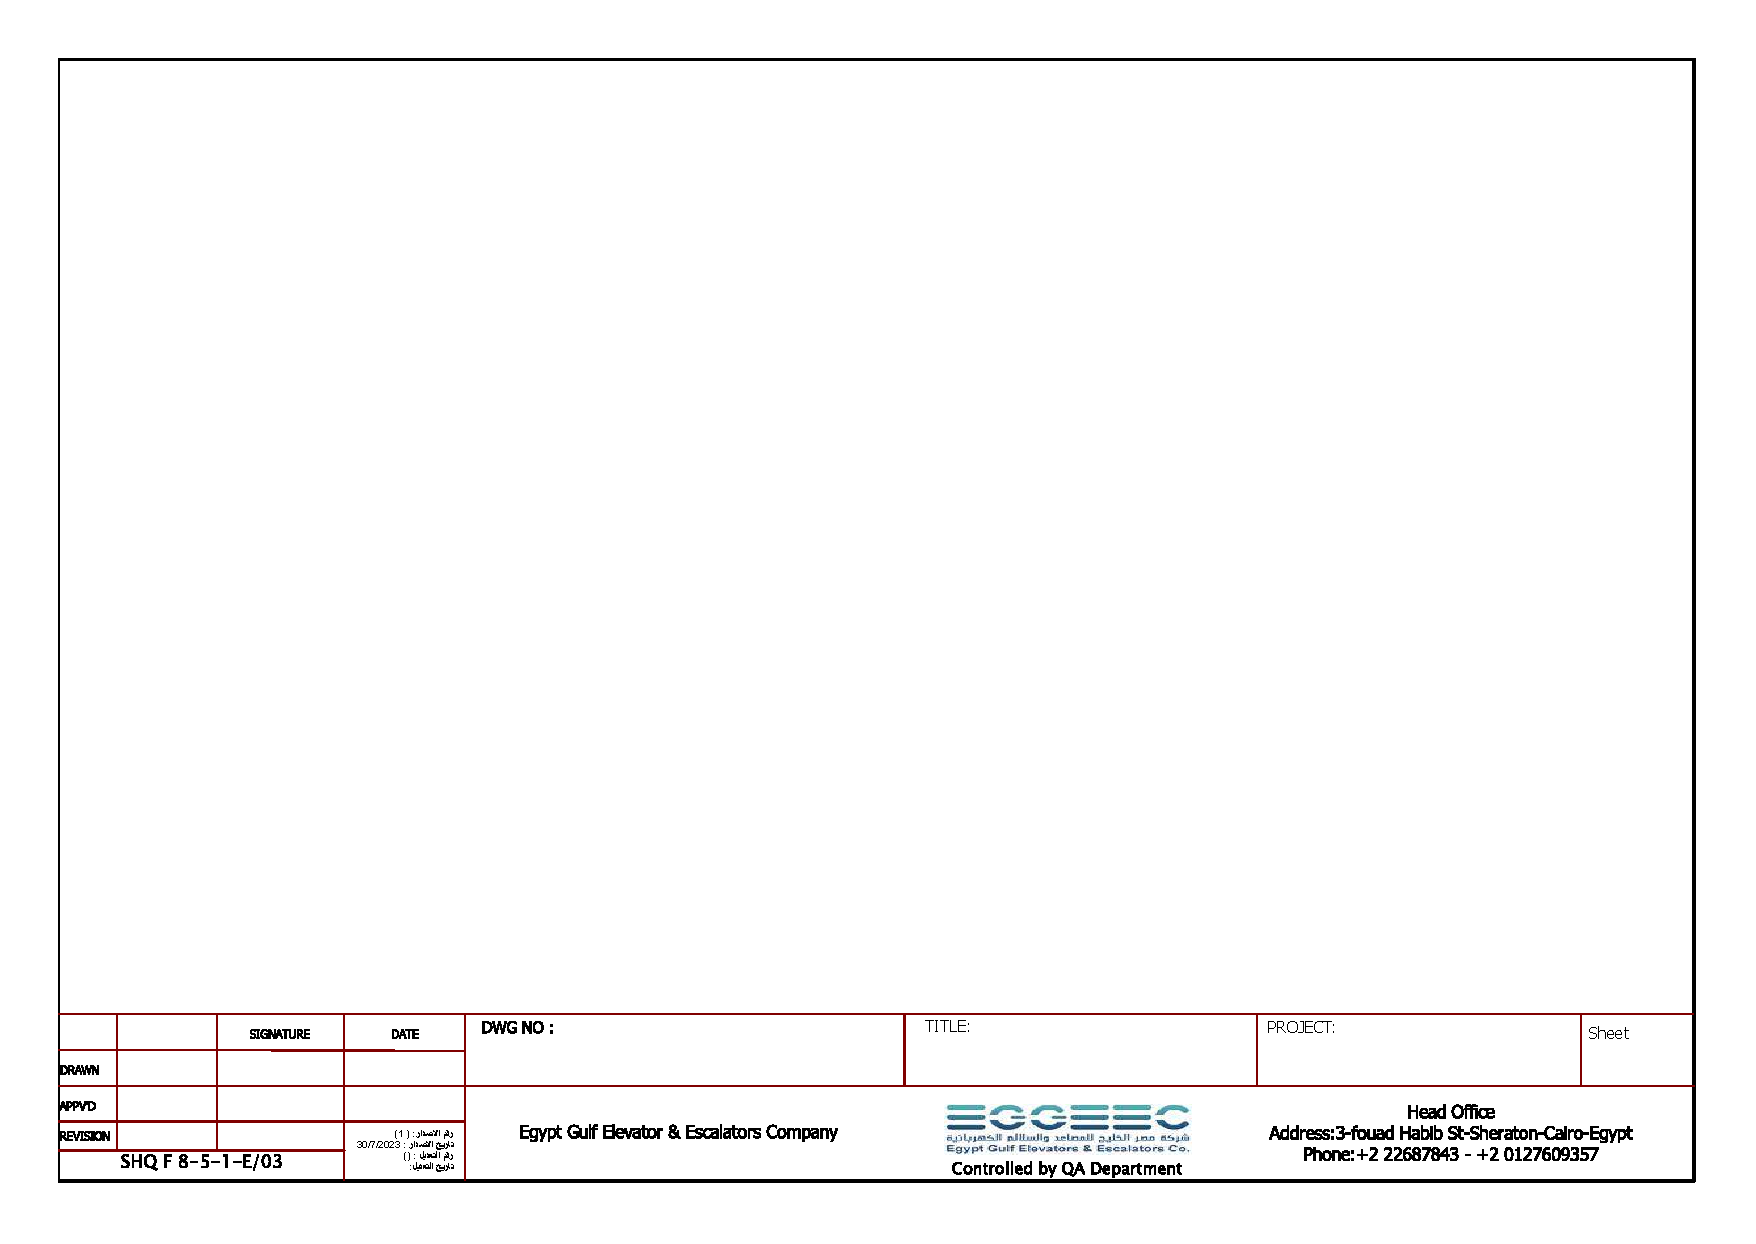
\includegraphics[scale=1]{drawings/drawing-1.pdf}};
	\node [inner sep = 0pt,anchor=west,scale=0.6] at 
	($(my-page.south west) + (2.1213cm,2.917cm)$){%
		M. Abdelmotalib%
	};
	\node [inner sep = 0pt,anchor=west,scale=0.6] at 
	($(my-page.south west) + (2.1213cm,2.3125cm)$){%
		Ahmed Farag%
	};
	\node [inner sep = 0pt,anchor=base,scale=0.85,color=red] at 
	($(my-page.south west) + (11.4647cm,3.1332cm)$){%
		\mydwgno%
	};
	\node [inner sep = 0pt,anchor=base,scale=0.85,color=red] at 
	($(my-page.south west) + (18.4765cm,3.1332cm)$){%
		\mytitle%
	};
	\node [inner sep = 0pt,anchor=base,scale=0.85,color=red] at 
	($(my-page.south west) + (24.0324cm,3.1332cm)$){%
		\myproject%
	};
	\node [inner sep = 0pt,anchor=base,scale=0.9] at 
	($(my-page.south west) + (27.7170cm,2.9167cm)$){%
		\stepcounter{PAGE}%
		\textbf{\thePAGE /\mytotalpage%		
		}%
	};
	\coordinate (my page left) at ($(my-page.south west) + (0,11.9141cm)$);
	\coordinate (paper center) at (current bounding box.center |- my page left);
		+b}
	{\end{tikzpicture}}

\newcommand{\myanno}[3][black]{\tikz[baseline=(A.base)]{
\node [text = white] (A) {#2};
\node [anchor = base west,minimum width=1em,text=#1] (B) at (A.base east) {#3};
\begin{scope}[on background layer]
	\coordinate (up) at (current bounding box.north);
	\coordinate (down) at (current bounding box.south);
	\fill[#1] (A.west |- up) rectangle (A.east |- down);
	\draw[#1](A.west |- up) rectangle (B.east |- down);
\end{scope}
}}

\newcommand{\myannothick}[3][black]{\tikz[baseline=(A.base)]{
\node [text = black] (A) {#2};
\node [anchor = base west,minimum width=1em,text=#1] (B) at (A.base east) {#3};
\begin{scope}[on background layer]
	\coordinate (up) at (current bounding box.north);
	\coordinate (down) at (current bounding box.south);
	\fill[
	pattern={Lines[
                  distance=2mm,
                  angle=45,
                  line width=0.7mm
                 ]},
        pattern color=#1!15	
	] (A.west |- up) rectangle (A.east |- down);
	\draw[#1!30](A.west |- up) rectangle (B.east |- down);
\end{scope}
}}

\begin{document}

\begin{drawingpage}[title = {Control Panel layout}]
	\node [scale =0.2,rotate = 90] at (paper center) {\includegraphics[scale=1]{drawings/Board 3.pdf}};
\end{drawingpage}


\begin{drawingpage}[title = {Circuit Breakers \& Rectifiers}]
	\node [scale =0.9] at (paper center) {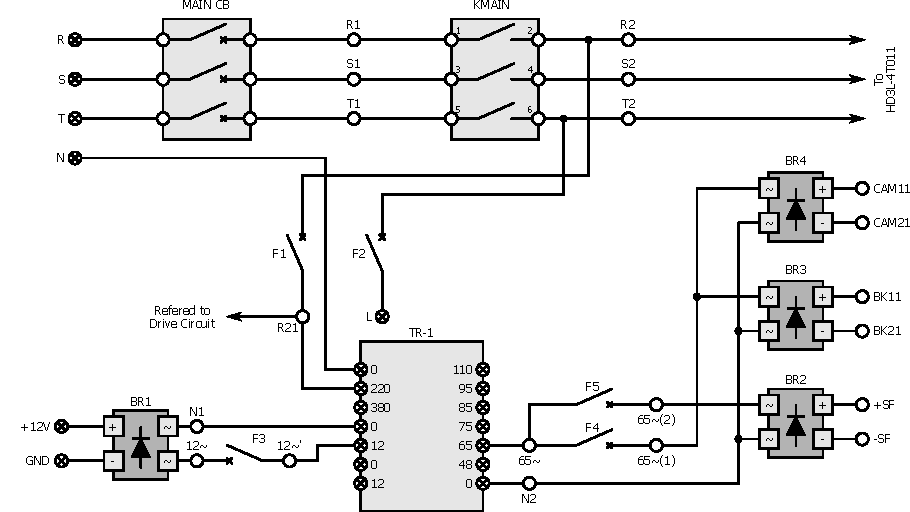
\includegraphics[scale=1]{drawings/1- Circuit Breakers (proj 2).pdf}};
\end{drawingpage}

\begin{drawingpage}[title = {Motor Drive wiring}]
	\node [scale =0.85] at (paper center) {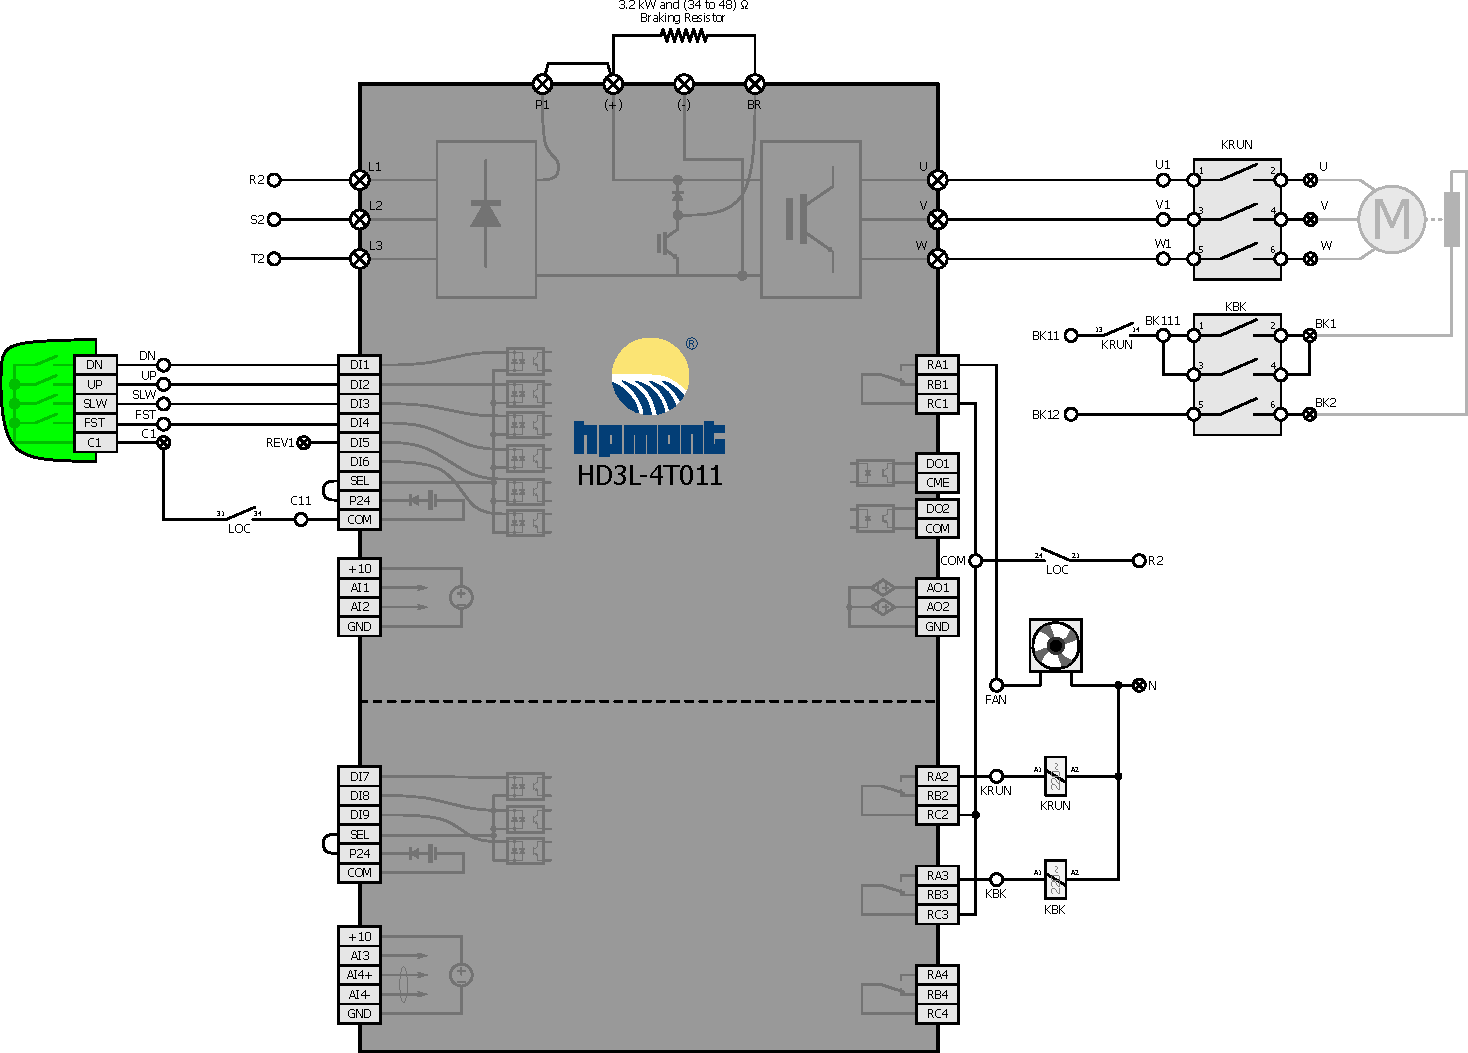
\includegraphics[scale=1]{drawings/2- Drive Circuits(proj 3 - 1 - 1).pdf}};
\end{drawingpage}


\begin{drawingpage}[title = {main board wiring(semi-auto)}]
	\node [scale =1] at (paper center) {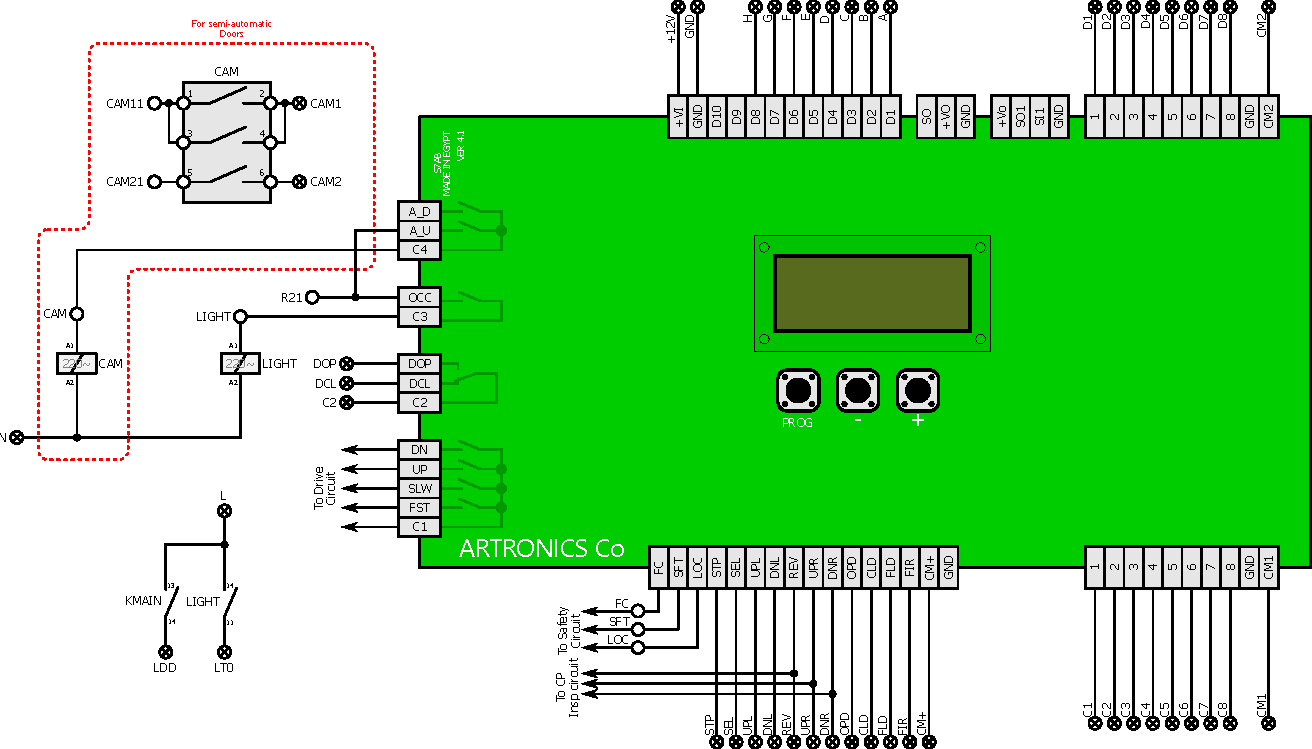
\includegraphics[scale=1]{drawings/4- artronic.pdf}};
\end{drawingpage}

\begin{drawingpage}[title = {Emergency Control Board}]
	\node [scale =1] at (paper center) {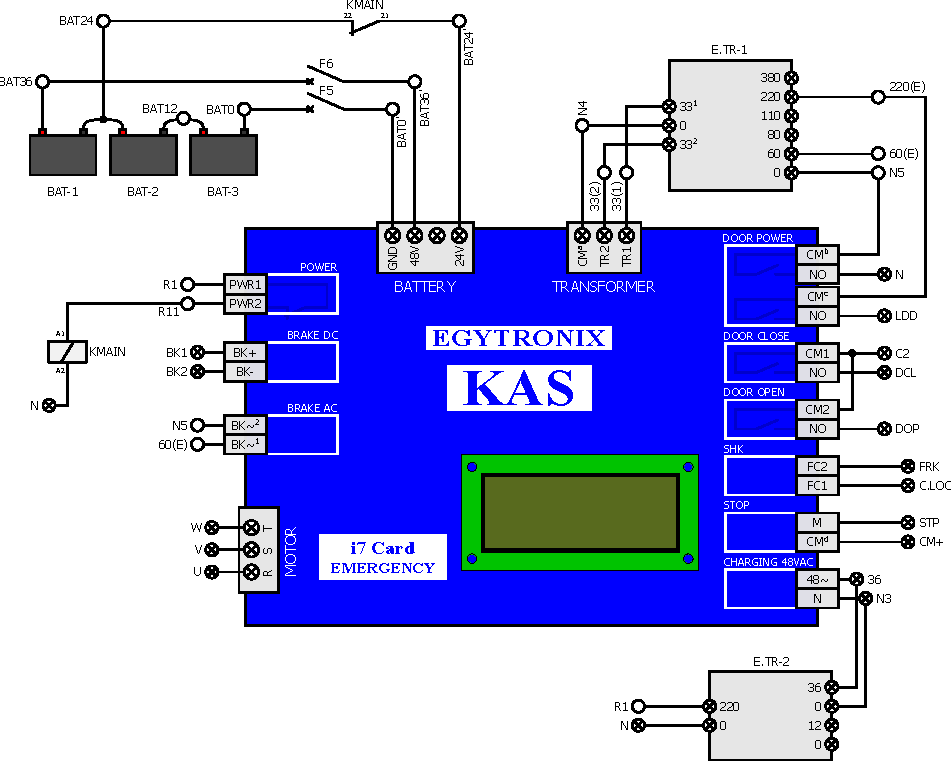
\includegraphics[scale=1]{drawings/emergency control.pdf}};
\end{drawingpage}

%
\begin{drawingpage}[title = {Terminal blocks}]
	\node [anchor=south,scale = 0.9] at (paper center) {%
	\begin{tblr}{colspec={|c|},cell{1}{1}={bg=red!30!black,fg=white}} \hline
	main terminal block \\ 
	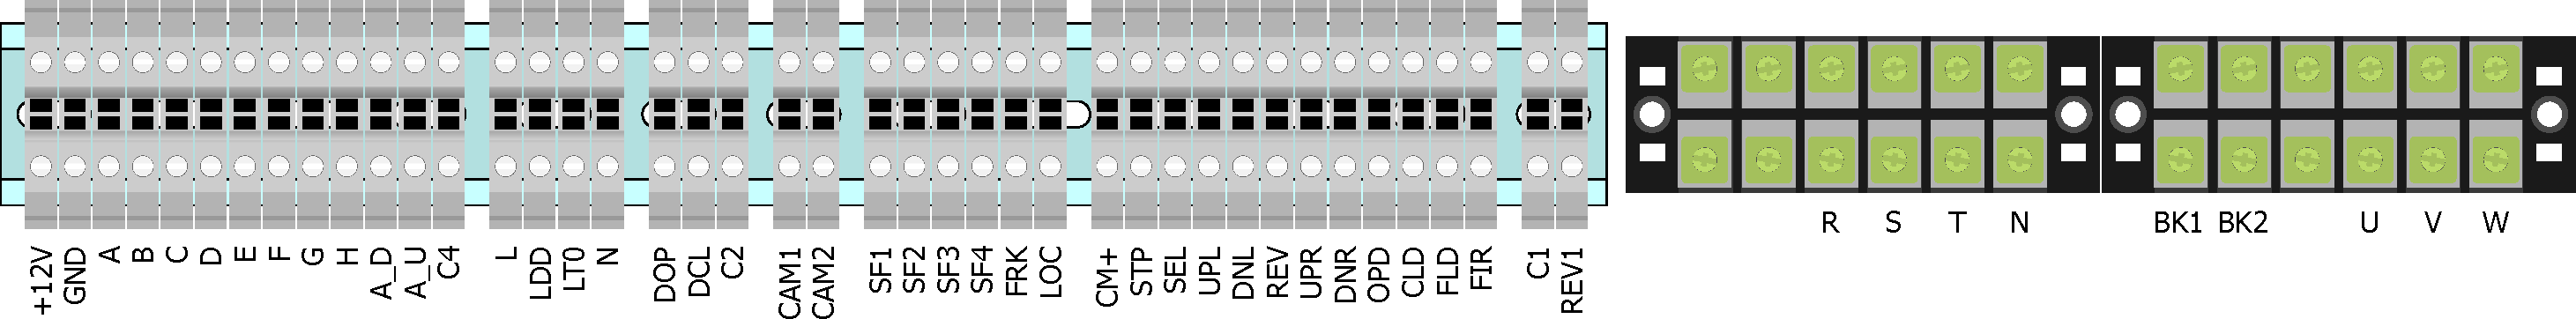
\includegraphics[scale=0.55]{drawings/5- terminals.pdf} \\ \hline
	\end{tblr}
	};
	\node [anchor=north,scale =0.9] at (paper center) {%
	\begin{tblr}{colspec={|c|},cell{1}{1}={bg=red!30!black,fg=white}} \hline
	Side terminal block \\ 
	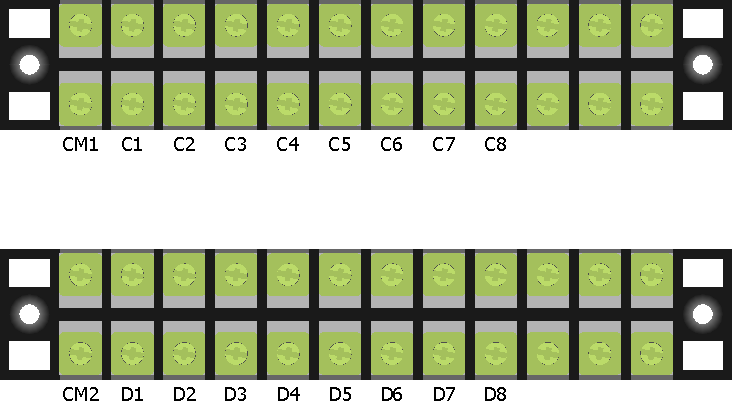
\includegraphics[scale=0.55]{drawings/5- terminals (prt 2).pdf} \\ \hline
	\end{tblr}
	};;
\end{drawingpage}

\begin{drawingpage}[title = {Safety Circuit}]
	\node [scale =0.9] at (paper center) {
		\begin{tblr}{colspec={|c||c|},cell{1}{1,2}={bg=red!30!black,fg=white}}
			Safety Circuit & Safety relays o/p with inspection circuit \\
			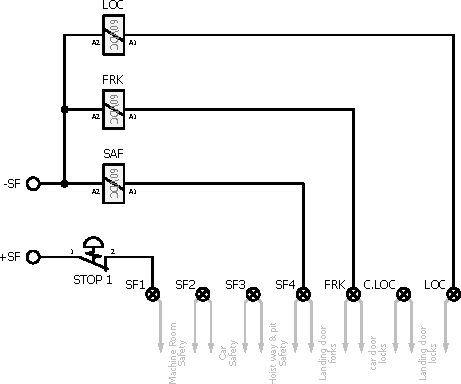
\includegraphics[scale=1]{drawings/6- Safety Circuit.pdf} & 
			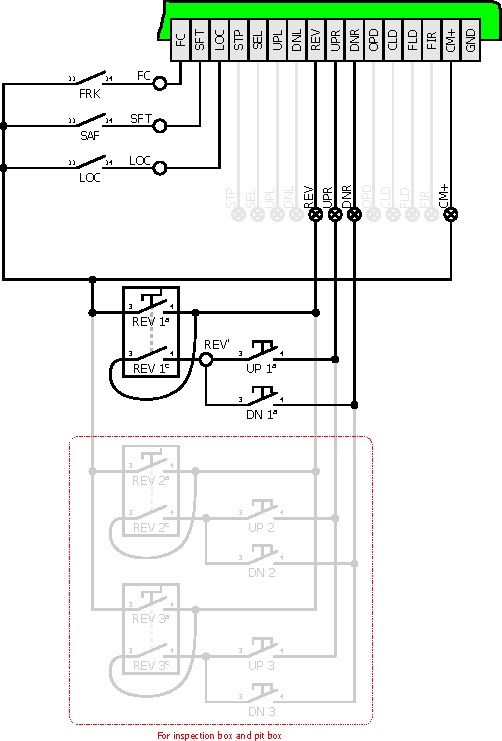
\includegraphics[scale=1]{drawings/safety circuit 2.pdf}
			\\ \hline
		\end{tblr}
	};
\end{drawingpage}

\begin{drawingpage}[title = {Wire labels (prt 1)}]
	\node [scale=0.82] at (paper center) {
		\parbox[t]{14cm}{\noindent%
		\begin{tblr}[evaluate=\fileInput]{colspec={|Q[c,m]|Q[h]|Q[c,m]|Q[c,1]|Q[c,m]|},
			cell{1}{1-Z}={bg=red!30!black,fg=white},
			measure = vbox,
			%cell{2}{2,3}={r=3,c=1}{},
			%cell{5}{2,3}={r=3,c=1}{},
			hline{3-Z}={1}{-}{},
			,baseline=t
		}
			Label & Location & N & Description & check\\ \hline
			\fileInput{table 1.tex}
		\end{tblr}}
		\parbox[t]{14cm}{\noindent%
		\begin{tblr}[evaluate=\fileInput]{colspec={|Q[c,m]|Q[h]|Q[c,m]|Q[c,1]|Q[c,m]|},
			cell{1}{1-Z}={bg=red!30!black,fg=white},
			measure = vbox,
			%cell{2}{2,3}={r=3,c=1}{},
			%cell{5}{2,3}={r=3,c=1}{},
			hline{3-Z}={1}{-}{},
			,baseline=t
		}
			Label & Location & N & Description & check\\ \hline
			\fileInput{table 2.tex}
		\end{tblr}}
	};
\end{drawingpage}
	
	
	\begin{drawingpage}[title = {Wire labels (prt 1)}]
	\node [scale=0.82] at (paper center) {
		\parbox[t]{14cm}{\noindent%
		\begin{tblr}[evaluate=\fileInput]{colspec={|Q[c,m]|Q[h]|Q[c,m]|Q[c,1]|Q[c,m]|},
			cell{1}{1-Z}={bg=red!30!black,fg=white},
			measure = vbox,
			%cell{2}{2,3}={r=3,c=1}{},
			%cell{5}{2,3}={r=3,c=1}{},
			hline{3-Z}={1}{-}{},
			,baseline=t
		}
			Label & Location & N & Description & check\\ \hline
			\fileInput{table 3.tex}
		\end{tblr}}
		\parbox[t]{14cm}{\noindent%
		\begin{tblr}[evaluate=\fileInput]{colspec={|Q[c,m]|Q[h]|Q[c,m]|Q[c,1,m]|Q[c,m]|},
			cell{1}{1-Z}={bg=red!30!black,fg=white},
			measure = vbox,
			%cell{2}{2,3}={r=3,c=1}{},
			%cell{5}{2,3}={r=3,c=1}{},
			hline{3-Z}={1}{-}{},
			,baseline=t
		}
			Label & Location & N & Description & check\\ \hline
			%\fileInput{table 3.tex}
		\end{tblr}}
	\savedata};
\end{drawingpage}

\end{document}
%latexmk -e "$pdflatex=q/pdflatex -synctex=1 -interaction=nonstopmode/" -pdf %.tex